We describe our learning strategy in \cref{sec:learning_strategy} (\cref{fig:diagram_ijcars})
and introduce our \ac{RC} simulation in \cref{sec:simulation}.

\begin{figure}
  \centering
  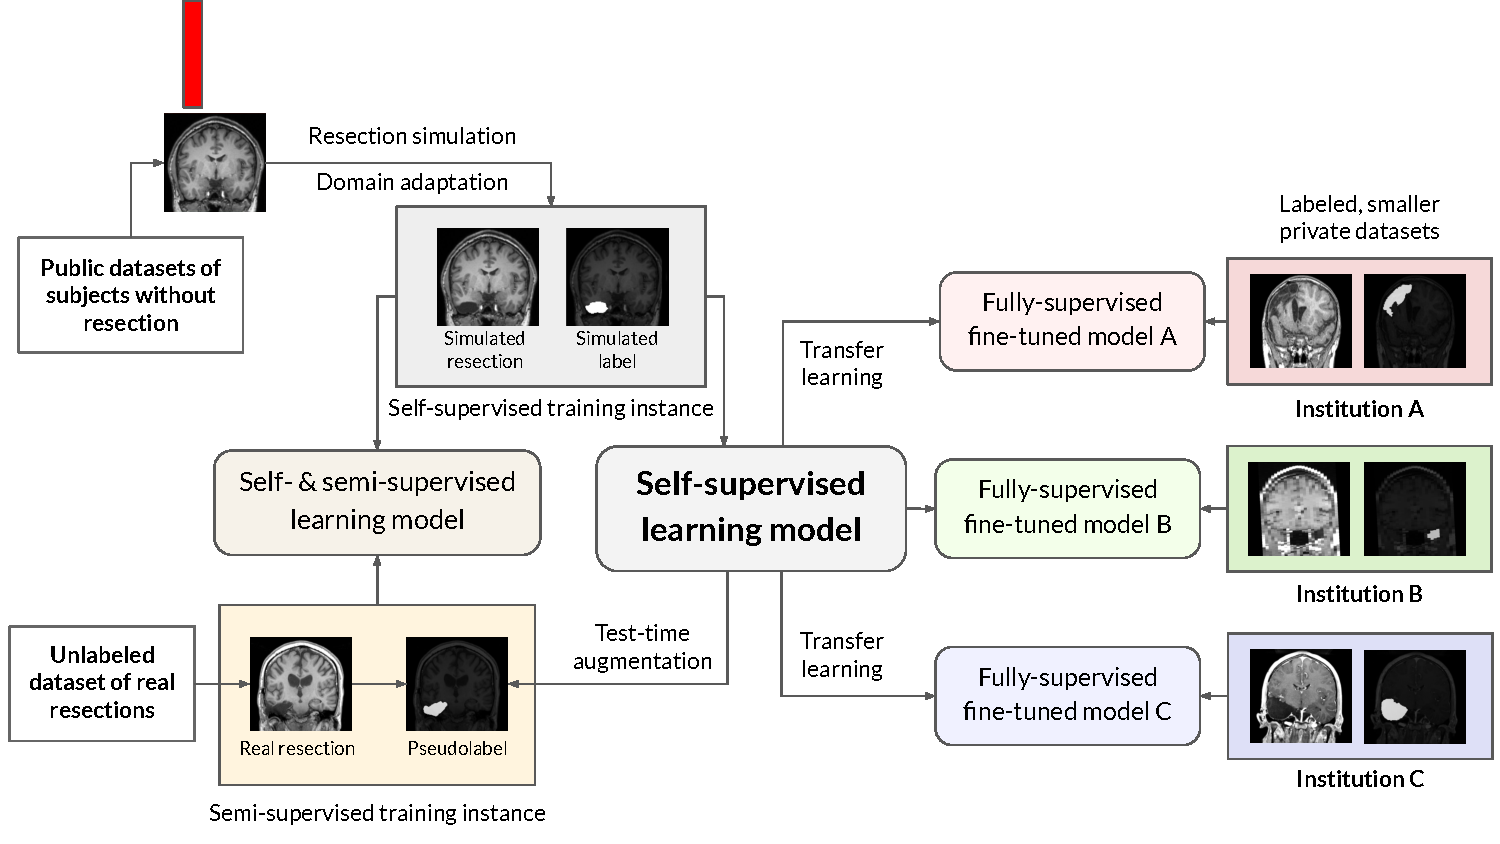
\includegraphics[trim={0 0 0 52},clip, width=\linewidth]{diagram_ijcars}
  \caption[Learning strategies for cavity segmentation]{
    Learning strategies.
    3D images without resections (top left) are modified by our resection simulation method to mimic postoperative images and their corresponding labels, generating training instances.
    These instances are used to train a baseline model in a self-supervised manner (middle).
    The baseline model generates pseudolabels from unlabeled images of patients who underwent resective surgery (bottom left).
    Instances from the \ac{RC} simulation and pseudolabeled dataset are used to train a new model in a self- and semi-supervised learning approach (left).
    The baseline model may be fine-tuned to improve its performance on small labeled datasets containing real resections from a single institution, using a standard fully-supervised learning approach (right).
  }
  \label{fig:diagram_ijcars}
\end{figure}
